% New Template!
% !TEX root = DesignDocument.tex


\chapter{System  and Unit Testing}
%%This section describes the approach taken with regard to system and unit testing. 
Testing for our project inluded mainly testing aspects of our hardware. Future sprints will include testing for the software we design as our message passing protocol over USB or GPIO pins, but for the first three sprints our goal was to chose the most efficient hardware and benchmark the amount of gigaflops able to be produced by the cluster, and how much the Ethernet network slows down the system. To accomplish this, we tested the physical capabilities of the hardware.

\section{Overview}
%%Provides a brief overview of the testing approach, testing frameworks, and general how testing is/will be done to provide a measure of success for the system. 

%%Each requirement (user story component) should be tested.    A review of objectives andconstraints might be needed here.  

We first tested the computational speed of the ODROID XU4 and Raspberry PI 2B. We then tested the amount of power used by each device with a voltimeter. From these tests, the ODROID produced more gigaflops per watt per dollar, influencing our choice to build our cluster out of ODROID XU4s.

\section{Dependencies}
%%Describe the basic dependencies which should include unit testing frameworks and reference material. 
To test the gigaflops of the cluster, we build and used LINPACK. This tool depends on several different pieces of software. First, it relies on some implementation of MPI, either OpenMPI or MPICH. We chose to use OpenMPI, which is installible as a standard debian package through the Ubuntu repositories. It also relies on either ATLAS or BLAS, Automatically Tuned Linear Algebra Software, or Basic Linear Algebra Subprograms, to be able to run it's linear algebra tests. We chose to use ATLAS, and built it from source for ARM on our machine. To test the Ethernet speed, the tool iperf was used.

\section{Test Setup and Execution}
%%Describe how test cases were developed, setup, and executed.  This section can be extremely involved if a complete list of test cases was warranted for the system.   One approach is to list each requirement, module, or component and describe the test.

%%The unit tests are described here.
The first tests were to compare the ODROID XU4 and Raspberry Pi 2B. The computational speed was testing by writing a program in C++ to read two large arrays of floating point values into memory and compute four different computations accross the arrays; addition, multiplication, divison, and sine. We recorded how long it took each device to complete the calcuations, and used the timing as a point of comparision between the two devices. The power consumption during runtime was also tested using a voltimeter while the C++ code was executed. The amount of gigflops per watt per dollar was computed to favor the ODROID, influencing our decision to build the cluster out of them. \\

The next series of tests were the hardware capabilities of the ODROID xU4. The Ethernet speed was tested by using iperf on two nodes, which is a tool availible in the default debian repositories to test the connection speed over Ethernet. Also, a USB to Ethernet device was tested in the same way. Once we knew that information, we tested the amount of gigaflops as recorded by a reliable tool, LINPACK. To do this we had to download the source code, create a Makefile for the ARM architecture, and build the executable. Once done, we adjusted the settings to a square matrix of size 38,600, used 4 and 16 for the P and Q values that determine how many cores to run the code on, and ran the test.

\section{System Testing}

The most significant testing that occured was of the speed of the cluster as a whole. It was tested using High Performance LINPACK, an open source benchmarking tool used by the top 500 organization to test the performance of supercomputers. We built this tool ourselves using ATLAS, automatically tuned linear algebra softare, and OpenMPI. 

%%\section{System Integration Analysis}

\section{Risk Analysis}

For this project, there was little risk due to the goal being to gather information rather than to produce a final product. Therefore, even failures would be viewed as valuable knowledge for the Product Owner of Dr. Karlsson. Also, it was very unlikely to be a total failure. The worst case would be if no communication worked at all and we weren't even able to cluster the devices entirely. Even then, at least Dr. Karlsson would be able to have the hardware at the end. He would have \$1,200 of single board computers, a switch, and power supply assuming nothing was broken over the course of the project.

\section{Issues, Problems}

\subsection{Use of Cores}

There were several issues encountered with testing. First, getting the ODROIDs to use their A15 cores was a challenge. Each device has four A7 cores and four A15, where the A7s use less power but are less powerful. For our purposes, we would ideally use all eight on every device. However, when we ran the tool HTOP to look at which cores were actually being used in real time, and ran LINPACK, we noticed that the scheduler seemed to only want to use the A7s in most scenarios. This is likely because the operating system is coded to use the lower power cores as much as possible, since single board computers are usually used in situations where power consumption is a concern. This is not the case for this project, though. So we tried to make the kernel use the A15s, either instead of the A7s or ideally in parallel with them. \\

There were several ways we tried to accomplish this. First, we use the command line option --bind-by-core 8 when running LINPACK with OpenMPI. This command would force the operating system to assing one process to one core, up to eight cores. However, this returned an error message saying that there were not enough cores detected in the architecture. Apparently, when the kernel decides not to use the A15 cores, it completely shuts them down and hides them entirely from the user. For our situation, this is far from ideal. So, we tried to manually shut down the A7 cores. This worked to a degree, but it's not possible to power off core 0, which is an A7, and as such the scheduler would put all of the processes assigned to it on the same core. This only served to lower performance even further. \\

What did work was unfortunatly not due to any setting changed by the user. When the ODROIDs are first powered on, they seem to be willing to use the A15 cores for the first LINPACK run on the system. After that, even with no changes to the configuration of LINPACK, MPI or anything else they will switch back to using the A7s. Using this method we were able to get a few tests in with the A15 cores, which are shown in our results section, but we don't know how or why. We can't repeat the situation that leads to the A15s being used very easily or reliably.

\subsection{OpenMPI with multiple network interfaces}

Another issue we encountered was when we tried to benchmark the Ring and Hypercube topologies. As can be seen in Figure~\ref{fig:ring} and Figure~\ref{fig:cube}, for these topologies to be built each individual ODROID needs to have more than one network interface. We accomplished this by using USB to Ethernet devices with the USB 3.0 ports. Though these connections were slower than the built in 1 Gigabit Ethernet ports by a factor of two, they were still enough for us to at least build the cluter in those different topologies. \\

The topologies were built successfully, and communication through the cluter was accomplished. We were able to SSH from any one node to any other. We believed that that would be enough for us to run LINPACK using OpenMPI. However, we encountered an issue. The tests would appear to start, processes would get assigned to each node, but then the program would hang indefinitely without producing output or progressing in any notable way. After much frustration and searching, we finally learned that MPI does not work on devices with multiple network interfaces on the same local network. This is because MPI is configured to use all availible network interfaces to maximize efficiency, which creates an issue for our cluster. Since each node has a routing table telling it how to get to any other node, if MPI ignore that and uses the wrong interface an infinite loop can be created. For example, if Dopey is trying to reach Grumpy, which requires going through Sleepy, it should send it's packet of data to Sleepy. However, if MPI decides instead to use the other interface and send it's packet to Snow White, Snow White would then have the data and try and send it to Grumpy. In order to do that, it would look at it's routing table and see that the first hop should be to Dopey. So it would send the packet back to Dopey. That could continue with the same packet being sent back and forth indefinitely, with no error message being produced. \\

As far as possible solutions to this issue are concerned, we were not able to encounter any. The different topology testing was the last step of our project, and left us with little time to solve the problem before the end of the semester. In the future, any other student group, or Dr. Christer Karlsson himself, would be encouraged to try and find a way to benchmark the speed of the Ring and Hypercube topologies. This may entail finding a way to force MPI to use only the network interface that the routing table tells it to use, or changing the IP addresses in some way such that they various interfaces on the same devices are all on different networks, or some such other work around within the restrictions given by MPI. Or, another possibility would be to abandon MPI and as such LINPACK altogether and find another benchmarking method. This would likely be more difficult and MPI is frequently used for parallel processing, and finding a benchmark that does not use it but is still widely utilized enough to be a good tool to compare the cluster to other similar implementations. 

\begin{figure}[tbh]
	\caption{Ring topology.}
	\centering
		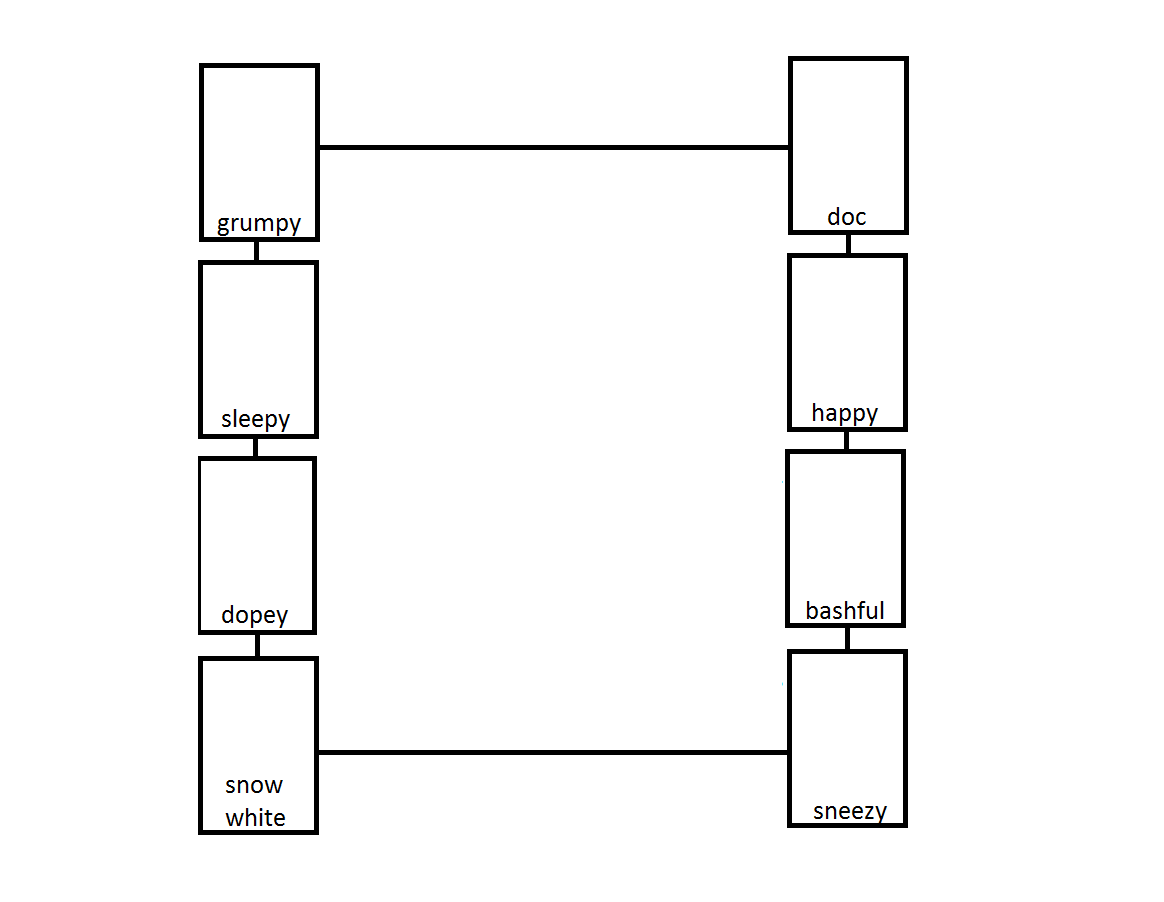
\includegraphics[width=0.75\textwidth]{ring.png}
	\label{fig:ring}
\end{figure}

\begin{figure}[tbh]
	\caption{Hypercube topology.}
	\centering
		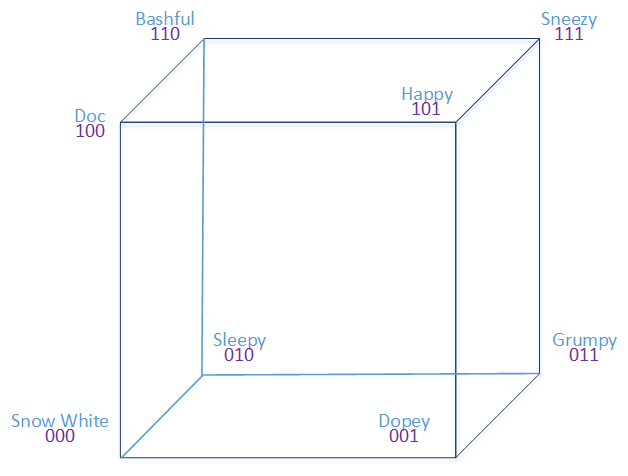
\includegraphics[width=0.75\textwidth]{HyperCube2.png}
	\label{fig:cube}
\end{figure}

\subsection{Changes to the Backlog}

Our final backlog changed over the course of the project. In the end, our goals going forward are as follows:

\begin{itemize}
	\item Benchmark the cluster using all availible cores.
	\item Benchmark different topologies not using a switch.
	\item Use the cluster to solve real-world problems.
	\item Continue looking at different possible communication methods with GPIO.
\end{itemize}



